\documentclass[twoside]{article}
\usepackage[utf8]{inputenc}
\usepackage[croatian]{babel}
\usepackage{array}
\usepackage{amsmath}
\usepackage{lmodern}
\usepackage[normalem]{ulem}
\usepackage{amssymb}
\usepackage{tabularx}
\usepackage{csquotes}
\usepackage{graphicx}
\usepackage{adjustbox}
\usepackage{float}
\usepackage[most]{tcolorbox}
\restylefloat{table}
\usepackage[shortlabels]{enumitem}
\usepackage{fancyhdr}
\fancypagestyle{mypagestyle}{
  \fancyhf{}
  \fancyhead[OC]{Problem mjerenja u kvantnoj mehanici}
  \fancyhead[EC]{Duje Štolfa}
  \fancyfoot[C]{\thepage}
  \renewcommand{\headrulewidth}{.4pt}
}
\pagestyle{mypagestyle}

\title{Problem mjerenja u kvantnoj mehanici}

\author{Duje Štolfa}


\begin{document}

\maketitle

\newtcolorbox{Sažetak}[1][]{enhanced,
  before skip=2mm,after skip=3mm,
  boxrule=0.4pt,left=5mm,right=2mm,top=1mm,bottom=1mm,
  colback=gray!20,
  colframe=gray!20!black,
  sharp corners,rounded corners=southeast,arc is angular,arc=3mm,
 #1}


\begin{Sažetak}
\subsubsection*{Sažetak}
Cilj je ovog eseja opisati problem mjerenja u kvantnoj mehanici i prikazati tri različita pokusa koji tu teoriju bilo osporavaju, bilo podržavaju te analizirati ih preko realističke i antirealističke interpretacije kvantne mehanike. U konačnici će ti zaključci dovesti do argumenta za izdvajanje bolje, uvjerljivije, od tih dvaju teorija.

\paragraph{Ključne riječi:} problem mjerenja, fizika, kvantna mehanika, Schrödingerova mačka, Wignerov prijatelj, pokus s dvije pukotine, realizam, antirealizam
\end{Sažetak}

\section{Uvod}
Kvantna se fizika počela razvijati početkom 20. stoljeća, a proučava sustave atomskih i subatomskih dimenzija koje opisuje valnim funkcijama \cite{Squires2020}. Valna funkcija nekog sustava, primjerice neke čestice, matematički opisuje tu česticu, a njena nam vrijednost ukazuje vjerojatnost pronalaska te čestice na nekom mjestu. Označava se velikim grčkim slovom psi $\Psi $ \cite{Britannica2020}. Kroz esej ću često naizmjenice koristiti izraze izmjeriti, očitati, promotriti i sl. jer u ovom kontekstu znače isto – izvršiti mjerenje. Bitna karakteristika mjerenja je da nužno mora imati utjecaj na sustav koji se mjeri; koliko god taj utjecaj bio malen, on će uvijek postojati \cite{Cushing2006}.

Ovim ću esejom analizirati kvantni problem mjerenja kroz tri pokusa iz povijesti kvantne mehanike: Schrödingerov Gedankenexperiment\footnote{Misaoni eksperiment. Pojam prvi put upotrebljava Albert Einstein pri opisivanju svog konceptualnog, za razliku od onog eksperimentalnog, pristupa pri oblikovanju teorije relativnosti. \cite{Perkowitz2010}} s mačkom, problem Wignerovog prijatelja i pokus s dvije pukotine. U prvom ću dijelu zasebno predstaviti svaki od pokusa, a u drugom usporedno analizirati rezultate tih pokusa kroz realističku i antirealističku interpretaciju valne funkcije te doći do odgovarajućeg zaključka.

\section{Schrödingerov Gedanekenexperiment s mačkom}
Erwin Schrödinger 1935. godine izdaje pregled i raspravu o tadašnjim spoznajama kvantne mehanike te opisuje sljedeći sustav:

\begin{displayquote}
Man kann auch ganz burleske Fälle konstruieren. Eine Katze wird in eine Stahlkammer gesperrt, zusammen mit folgender Höllenmaschine (die man gegen den direkten Zugriff der Katze sichern muß): in einem Geigerschen Zählrohr befindet sich eine winzige Menge radioaktiver Substanz, so wenig, daß im Laufe einer Stunde vielleicht eines von den Atomen zerfällt, ebenso wahrscheinlich aber auch keines; geschieht es, so spricht das Zählrohr an und betätigt über ein Relais ein Hämmerchen, das ein Kölbchen mit Blausäure zertrümmert.\cite{Schroedinger1935} 
\end{displayquote}

\begin{displayquote}
One can even set up quite ridiculous cases. A cat is penned up in a steel chamber, along with the following diabolical device (which must be secured against direct interference by the cat): in a Geiger counter there is a tiny bit of radioactive substance, so small, that perhaps in the course of one hour one of the atoms decays, but also, with equal probability, perhaps none; if it happens, the counter tube discharges and through a relay releases a hammer which shatters a small flask of hydrocyanic acid.\cite{Trimmer1980}
\end{displayquote}

\noindent
Ovaj je sustav kompozicija sustava mačke $\phi$ i atoma $\psi$, a kao takav se u kvantnoj mehanici modelira valnom funkcijom koja u trenutku t = 0 ima oblik:

\[\Psi(t=0) = \phi_{macka}\psi_{atom}\]
\noindent
Sustavi mačke i atoma sada su spregnuti\footnote{Kvantno sprezanje, svojstvo skupa kvantnih sustava, najčešće subatomskih čestica, u kojem je obilježje jednog sustava izravno i upravo povezano s istovjetnim svojstvima ostalih sustava, neovisno o razmještaju (prostornoj razdvojenosti) tih sustava. \cite{MerriamWebster}}, a razvoj valne funkcije cijelog sustava kroz vrijeme (tj. stanje sustava prije otvaranja komore) upravljan je Schrödingerovim jednadžbama i opisan valnom funkcijom

\[\Psi(t) = \alpha(t)\phi_{macka}\psi_{atom} + \beta(t)\phi_{uginula}\psi_{raspadnut}\]
\noindent
Ovakva valna funkcija predstavlja superpoziciju stanja žive mačke i neraspadnutog atoma te uginule mačke i raspadnutog atoma. Otvaranjem komore i očitavanjem (mjerenjem) stanja u kojem se nalaze mačka i radioaktivni atom, valna se funkcija urušava u to izmjereno stanje koje može biti ili \emph{mačka je živa, a atom se nije raspao} ili \emph{mačka je uginula, a atom se raspao}.


\section{Wignerov prijatelj}

Problem Wignerovog prijatelja opisuje sustav gdje Wigner\footnote{Eugene Wigner (1902.-1995.) fizičar rodom iz Budimpešte, zajedno sa J. Jensenom i M. Mayer dobitnik Nobelove nagrade za fiziku 1963. za istražiivanja u nuklearnoj fizici. Prvi put predstavlja ovaj Gedankenexperiment 1962. u časopisu „The Scientist Speculates“. \cite{Britannica2021}} promatra laboratorij u kojem njegov prijatelj promatra bilo kakav kvantni sustav, primjerice sustav iz Schrödingerovog misaonog eksperimenta, pri čemu Wigner može saznati stanje kvantnog sustava samo ako mu njegov prijatelj prenese taj podatak. U ovom slučaju laboratorij postaje kvantni sustav (u općem smislu), tj. poprima svojstva kvantnog sustava, i, kao takav, također je opisan valnom funkcijom.

Prije nego što Wignerov prijatelj izvrši mjerenje kvantnog sustava, za Wignera je laboratorij u superpoziciji stanja \emph{prijatelj je izmjerio živu mačku i mačka je živa} te \emph{prijatelj je izmjerio uginulu mačku i mačka je uginula}, a za njegovog je prijatelja kvantni sustav s mačkom u superpoziciji stanja žive i uginule mačke. 

U ovakvom okruženju, valna funkcija kvantnog sustava urušit će se u trenutku kada Wignerov prijatelj izvrši mjerenje, a valna funkcija laboratorija kada prijatelj tu informaciju prenese Wigneru.


\section{Pokus s dvije pukotine}

Prvi pokus s dvije pukotine proveo je Thomas Young 1800. godine \cite{Young2015} i spoznao da svjetlost propuštena kroz dvije pukotine na zastoru iza njih formira, umjesto očekivane dvije svijetle pruge, niz usporednih tamnih i svijetlih linija. Young je iz ovog pokusa zaključio da se svjetlost ponaša kao val (što će se kroz 19. i 20. stoljeće kristalizirati u valno-čestičnu definiciju svjetlosti) i da može konstruktivno ili destruktivno interferirati s drugim valovima svjetlosti, što se na zastoru očituje kao svijetle, odnosno tamne linije. 

\begin{figure}[!htb]
    \centering
    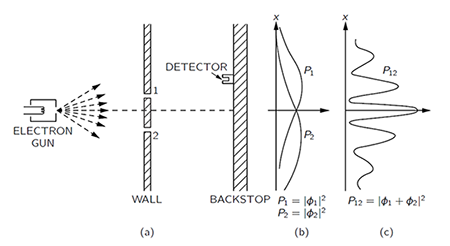
\includegraphics{eksperiment-1}
    \caption{Pokus s dvije pukotine \cite{Cushing2006}}
    \label{eksperiment1}
    \end{figure}

Youngov pokus prikazuje svojstva svjetlosti kao dio optike, dok drugačija inačica tog pokusa prikazuje kvantno-mehaničke principe. Pokus s dvije pukotine kakvog opisuju Feynman, Leighton i Sands \cite{Feynman2010} postavljen je tako da se ispred elektronskog topa nalazi pregrada s dvije pukotine iza koje je zid s pomičnim detektorom elektrona. Elektronski top usmjerimo prema pukotinama i pomičući detektor bilježimo prosječnu stopu očitavanja elektrona za svaku udaljenost $x$ od sredine zida. Kako elektronski top ispušta elektrone u jednakim vremenskim intervalima, vjerojatnost da ćemo na nekoj udaljenosti $x$ detektirati elektron $P_{12}$  bit će razmjerna zabilježenoj stopi za taj $x$. Krivulja na Slici \ref{eksperiment1} rezultat je ovog pokusa.

Stavimo li još jedan detektor na zid na položaj $x$ različit od položaja prvog detektora, uočit ćemo da se očitavanja detektora nikad ne događaju istovremeno. Dakle, u jednom trenutku kroz neku od dvije pukotine može proći samo jedan elektron. Možemo pretpostaviti sljedeće:
\begin{displayquote}
\emph{Pretpostavka A:} Elektron koji prolazi kroz pukotine prođe \emph{ili} kroz pukotinu 1 \emph{ili} kroz pukotinu 2.
\end{displayquote}
Dakle, ukupan broj očitavanja elektrona za svako mjesto $x$ mora biti jednak zbroju broja elektrona koji su na taj $x$ došli prolazeći kroz pukotinu 1 i broja elektrona koji su na taj $x$ došli prolazeći kroz pukotinu 2. Analogno tome, vjerojatnost da ćemo na nekoj udaljenosti $x$ detektirati elektron koji je prošao \emph{ili kroz pukotinu 1 ili kroz pukotinu 2} ($P_{12}$ ) mora biti jednaka zbroju istih vjerojatnosti $P_1$ i $P_2$ za pukotinu 1 i pukotinu 2.
\[ P_{12} = P_1 + P_2\]
Kako bismo izračunali vjerojatnosti $P_1$ i $P_2$ moramo za svaki x odrediti koliko je elektrona došlo iz prve, a koliko iz druge pukotine, tj. moramo odrediti kroz koju je pukotinu prošao svaki elektron. Ovo se može napraviti na sljedeće načine:

\begin{enumerate}[label={(\arabic*)}]
    \item \textbf{Propuštanje elektrona kroz jednu po jednu pukotinu}

Prekrivanjem (zatvaranjem) jedne od pukotina možemo prebrojati koliko je elektrona došlo na položaj $x$ iz druge neprekrivene pukotine. Ovo vrijedi jer \emph{pretpostavka A}  podrazumijeva da prolazak elektrona kroz neku pukotinu nije ovisan o prekrivenosti preostale pukotine, tj. ako je elektron prošao kroz pukotinu 1 dok je pukotina 2 bila otkrivena, prošao bi kroz nju i da je pukotina 2 bila prekrivena.

Krivulje $P_1$ i $P_2$ na (b) dijelu Slike \ref{eksperiment1} vjerojatnosti su detektiranja elektrona kada je u pokusu bila prekrivena pukotina 2 odnosno pukotina 1. Kao što se može zaključiti uspoređivanjem dijelova (b) i (c) na Slici \ref{eksperiment1}, zbrajanjem ovih vjerojatnosti ne dobivamo istu vjerojatnost koju smo dobili kada su obje pukotine bile otkrivene, tj.
\[ P_{12} \neq P_1 + P_2\]
Kako ukupan broj elektrona koji je došao na neki položaj $x$ nije jednak zbroju broja elektrona koji su na taj $x$ došli prolazeći kroz pukotinu 1 i broja elektrona koji su na taj $x$ došli prolazeći kroz pukotinu 2, kao što implicira \emph{pretpostavka A}, zaključujemo da \emph{pretpostavka A} ne smije biti slučaj.
    \item \textbf{Promatranje elektrona pri prolazu kroz pukotine.}

\begin{figure}[!htb]
    \centering
    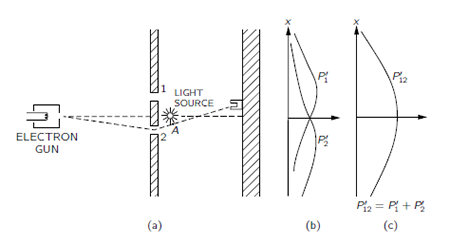
\includegraphics{eksperiment-2}
    \caption{Promatranje elektona pri prolasku kroz pukotine \cite{Cushing2006}}
    \label{eksperiment2}
    \end{figure}

Elektrone možemo promatrati na tako da vrlo jak izvor svjetlosti smjestimo odmah iza pregrade; kako elektroni prolaze kroz pukotine, svjetlost se reflektira od njih, što osoba koja izvodi pokus vidi kao bljesak svjetlosti u blizini pukotine kroz koju je elektron prošao. Provedbom pokusa uočava se da svaku detekciju elektrona prati bljesak ili na pukotini 1 ili na pukotini 2, nikada na obje pukotine istovremeno. Ovime smo empirijski potvrdili \emph{pretpostavku A}. 

Prebrojavanjem elektrona koji su detektirani na položaju x i koji su prošli kroz pukotinu 1 odnosno pukotinu 2 možemo izračunati vjerojatnosti detekcije elektrona na tom položaju ako je prošao kroz pukotinu 1 ($P_1^{'}$), pukotinu 2 ($P_2^{'}$) ili kroz bilo koju od te dvije pukotine ($P_{12}^{'}$). Na dijelu (b) na Slici 2 vidimo da vjerojatnosti $P_1^{'}$ i $P_2^{'}$ odgovaraju vjerojatnostima $P_1$ i $P_2$ iz slučaja (1), dok je $P_{12}^{'} \neq P_{12}$. Zbrojimo li vjerojatnosti $P_1^{'}$ i $P_2^{'}$ dobit ćemo $P_{12}^{'}$, kao što je bilo očekivano da će se dogoditi u slučaju (1).

\end{enumerate}

\section{Rasprava}
Početkom 20. stoljeća, kada je kvantna teorija još bila u svojim začetcima, vodile su se rasprave o konzistentnosti kvantne mehanike i o tome u kojoj mjeri ona opisuje stvarnost. Tim je raspravama skrenuta pozornost na nekonzistentnosti koje su tada bile postojale u kvantnoj teoriji (koje za današnju teoriju nisu značajne jer su tim raspravama one i uklonjene) \cite{Cushing2006}, dok se znanstvene teorije o odgovoru na potonji problem nisu ni do danas usuglasile. U znanstvenoj se zajednici tako mogu uočiti dvije škole misli: Einsteinova realistička i Bohrova antirealistička \cite{Cushing2006}. Naime, ta se razdioba može svesti na to kako interpretiramo valnu funkciju:
\begin{displayquote}
\emph{Interpretacija 1:} Valna je funcija stvaran opis nekog kvantnog sustava.

\emph{Interpretacija 2:} Valna funkcija samo je sadržaj našeg znanja o nekom kvatnom sustavu.
\end{displayquote}
pri čemu zauzimamo realistički odnosno antirealistički stav. Ovo nesuglasje uočio je i Einstein te ga spominje u pismu Heisenbergu:

\begin{displayquote}
If one attempts to interpret the $\Psi$-function as a complete description of a state, independent of whether or not it is observed, then this means that at the time in question the cat is neither alive nor pulverized. But one or the other situation would be realized by making an observation. If one rejects this interpretation then one must assume the $\Psi$-function does not express the real situation but rather that it expresses the contents of our knowledge of the situation. This is Born's interpretation, which most theorists today probably share. But then the laws of nature that one can formulate do not apply to the change with time of something that exists, but rather to the time variation of the content of our legitimate expectations. Both points of view are logically unobjectionable; but I cannot believe that either of these viewpoints will finally be established.\cite{Przibram1967}
\end{displayquote}

\noindent
Analizirajmo tri prethodno objašnjena pokusa razmatrajući realističke i antirealističke interpretacije tih pokusa.

\subsection{Schrödingerov Gedanekenexperiment s mačkom}
Uzmemo li valnu funkciju kao potpun opis sustava komore s mačkom moramo zaključiti da mačka ne ugiba, niti je živa, sve do trenutka kada dođe do urušavanja valne funkcije, tj. kada se na sustavu izvršimo mjerenje. Drugim riječima, ako otvaranjem komore promatrač vidi uginulu mačku, ona upravo tada i ugiba iako se atom mogao raspasti dugo prije otvaranja komore. Dakle, da bismo prihvatili \emph{interpretaciju 1}, otvaranje komore, a ne raspad atoma i ispuštanje otrovnog plina, mora biti uzrok smrti mačke. 

Do ovakvih neintuitivnih rezultata ne dolazimo kada valna funkcija predstavlja samo sadržaj promatračevog znanja o sustavu mačke i atoma; mačka može uginuti, a valna funkcija i dalje može biti u superpoziciji jer promatrač još nije napravio mjerenje. Mjerenjem promatrač samo revidira svoje znanje o tom sustavu koje se u tom trenutku uskladi sa stvarnim stanjem u komori.

\subsection{Wignerov prijatelj}
Kao i kod Schrödingerove mačke, ovaj misaoni eksperiment ukazuje na razlike između stvarnog stanja u laboratoriju i Wignerovog poimanja laboratorija preko valne funkcije. U opisanom trenutku nakon što je Wignerov prijatelj izvršio mjerenje, a prije nego što je rezultat tog mjerenja rekao Wigneru, stanje valne funkcije laboratorija\footnote{ \emph{laboratorij je u superpoziciji mogućih stanja}} ne opisuje stvarno stanje u laboratoriju\footnote{ \emph{prijatelj je očitao jedno od mogućih stanja i kvantni sustav je u tom očitanom stanju}}. Dakle, za sustav laboratorija \emph{interpretacija 1} ne može biti slučaj, a u \emph{interpretaciji 2} rezultati ovog pokusa intuitivno su prihvatljivi.

\subsection{Pokus s dvije pukotine}
Pokusom smo uočili da promatranje elektrona uzrokuje promjenu njihovog ponašanja i u konačnici mijenja rezultate pokusa. Zaključili smo da u slučaju u kojem elektroni nisu promatrani ne možemo reći da su prošli isključivo kroz jednu od pukotina, tj. elektroni su u superpoziciji stanja \emph{$e^-$ je prošao kroz pukotinu 1} i \emph{$e^-$ je prošao kroz pukotinu 2}. Dakle, valna funkcija elektrona predstavlja stvaran opis stanja elektrona, a urušavanje te valne funkcije prati i odgovarajuća promjena rezultata pokusa. Feynman Leighton i Sands daju jezgrovit odgovor na pitanje „Kroz koju je pukotinu prošao elektron?“, a samim time pojašnjavaju prirodu ponašanja sustava u superpoziciji: 

\begin{displayquote}
If one looks at the holes or, more accurately, if one has a piece of apparatus which is capable of determining whether the electrons go through hole 1 or hole 2, then one can say that it goes either through hole 1 or hole 2. But, when one does not try to tell which way the electron goes, when there is nothing in the experiment to disturb the electrons, then one may not say that an electron goes either through hole 1 or hole 2. If one does say that, and starts to make any deductions from the statement, he will make errors in the analysis. This is the logical tightrope on which we must walk if we wish to describe nature successfully.\cite{Feynman2010}
\end{displayquote}

\noindent
Jedna od zamjerki pokusu može biti da se korištenjem izrazito jakog izvora svjetlosti (što znači da fotoni imaju visoku energiju, odnosno veliku količinu gibanja) na elektrone utjecalo u toj mjeri da je došlo do značajne promjene u rezultatima pokusa i da je trebao biti korišten manje intenzivan izvor svjetlosti. Provedbom takvog pokusa \cite{Feynman2010} uočava se da smanjivanjem intenziteta svjetlosti smanjuje preciznost mjerenja, tj. dio elektrona detektiran je na zidu bez odgovarajućeg bljeska na ijednoj od pukotina, pri čemu se takvi neizmjereni elektroni gibaju kao i u pokusu bez izvora svjetlosti. Mijenjanjem intenziteta svjetlosti može se zaključiti da što je veći broj elektron za koje znamo kroz koju su pukotinu prošli, to će biti manji biti utjecaji interferencije\footnote{Pojam interferencije nije ograničen isključivo na pojave iz optike, već se njime može opisati i slučaj prethodno opisanog pokusa u kojem elektroni nisu bili promatrani}. U suštini, uočeni je princip inačica principa neodređenosti\footnote{Princip po kojem je od dvaju parametara, moguće precizno znati samo jednog. Primjerice, što preciznije čestici odredimo količinu gibanja $p$ to ćemo joj s manjom preciznošću moći odrediti položaj $x$ - $\sigma_p\sigma_x \geq \frac{\hbar}{2}$, gdje su $\sigma_p$ i $\sigma_x$ standardne devijacije količine gibanja odnosno položaja čestice, a $\hbar$ reducirana Planckova konstanta.} tipičnog za kopenhagensku\footnote{Kopenhagensko tumačenje kvantne mehanike bio je prvi opći pokušaj razumijevanja kvantne teorije. Njeni su proponenti Danski fizičari Niels Bohr, Werner Heisenberg i Max Born. \cite{Faye2019}} antirealističku interpretaciju kvantne mehanike.

\subsection{Osvrt na raspravu}
Schrödingerov pokus s mačkom i pokus s Wignerovim prijateljem argumenti su protiv \emph{interpretacije 1} valne funkcije. Da bi u njima \emph{interpretacija 1} mogla biti slučaj, u prvom bismo pokusu trebali prihvatiti da značajna promjena na sustavu, preciznije promjena na mački, može biti uzrokovana isključivo mjerenjem tog sustava, dok bismo za drugi slučaj trebali odbaciti ulogu Wignera kao promatrača, tj. pokazati da on ne može biti promatrač, zbog čega se laboratorij ne bi mogao opisati valnom funkcijom. 

Uz ovo, jedan od mogućih razloga zašto u navedenim eksperimentima dolazimo do nekonzistentnih rezultata je da kvantno-mehaničke zakonitosti ne moraju biti primjenjive na sustave koji nisu kvantnih dimenzija (kao što su mačka ili laboratorij). Dokazivanje ove tvrdnje podrazumijeva izračun te granice, tj. odgovor na pitanje „Ako postoji granica između kvantnog i ne kvantnog svijeta, koja je?“ U jednom je novijem istraživanju\cite{Frauchiger2018} provedena\footnote{Provedeni je pokus također Gedankenexperiment.}  inačica Wignerovog pokusa čiji su rezultati ukazali na upravo tu neprimjenjivost kvantnih zakona na kompleksne sustave velikih dimenzija, ali istraživanjem nije određena prethodno navedena granica. 

Bitnu različitost mikroskopskih i makroskopskih sustava, tj. činjenicu da u mikroskopskim sustavima kvantno-mehanički principi, kao što su oni koje prikazuje Schrödingerov Gedankenexperiment, mogu biti prihvatljivi, spominje i Cushing:

\begin{displayquote}
On the other hand, if the wave function represents the state of an individual cat (…) then a dramatic physical change in the cat accompanies the collapse of the wave function. While a sudden change of the physical state just by observation may not appear too bothersome at the microlevel, it is disturbing and appears highly improbable at the level of macroscopic systems, such as a cat. \cite{Cushing2006}
\end{displayquote}

\noindent
Argumenti, zaključci i pokusi predstavljeni u eseju koji djeluju u korist antirealističkoj interpretaciji kvantne teorije imaju, u suštini, dvije ključne mane. Oba su pokusa (Wignerov i Schrödingerov) misaoni eksperimenti, pa su zaključci iz tih pokusa, kao i pokusi sami, manje uvjerljivi od zaključka iz empirijskog pokusa s dvije pukotine, koji je kroz povijest kvantne teorije proveden više puta \cite{Feynman2010}. Druga je mana antirealističke interpretacije činjenica da prihvaćanjem interpretacije valne funkcije u kojoj je ona samo prikaz sadržaja našeg (promatračevog) znanja o kvantnom sustavu prihvaćamo (1) da postoje svojstva nekog sustava, odnosno pojave u svijetu, koja nikada ne možemo spoznati i (2) kvantna teorija ne govori ništa o svijetu, već samo o informacijama koje smo već spoznali. Potonja implikacija čini kvantnu teoriju u suštini beskorisnom. Heisenberg je uočio da su sve dosadašnje teorije fizike u nekoj mjeri opisivale svijet: 

\begin{displayquote}
In classical physics science started from the belief... that we could describe the world... without any reference to ourselves… Its success has led to the general ideal of an objective description of the world.\cite{Heisenberg1958}
\end{displayquote}

\noindent
Provedbom pokusa s dvije pukotine zaključeno je da, ako elektroni pri prolasku kroz pukotine nisu promatrani, ne možemo govoriti da su isključivo prošli ili kroz prvu ili kroz drugu pukotinu, već da moraju biti u superpoziciji ta dva stanja. Ova spoznaja daje potporu realističkom tumačenju valne funkcije jer predstavlja empirijski slučaj u kojem je kvantni sustav zaista u superpoziciji, odnosno u kojem kvantni sustav ne može ne biti u superpoziciji.

\section{Zaključak}
Pristup problemu mjerenja razdijelio je teoretičare na antirealiste, čiji je predstavnik bio Neils Bohr, koji prihvaćaju valnu funkciju samo kao sadržaj našeg znanja o nekom kvantnom sustavu, i realiste koji se slažu s mišljenjima Alberta Einsteina i koji prihvaćaju valnu funkciju kao prikaz stvarnog stanja kvantnog sustava. U eseju smo, preko analize rezultata dva Gedanken ili misaona i jednog empirijskog pokusa sa stavova realizma i antirealizma, pri čemu je empirijski pokus ukazao da nepromatrani elektron pri prolasku kroz dvije pukotine mora biti u superpoziciji, odnosno da u tom slučaju superpozicija odgovara stvarnom, fizičkom stanju sutava elektrona, pokazali da smo skloniji realističkoj interpretaciji kvantne mehanike.

\nocite{*}
\bibliography{bbliografija} 
\bibliographystyle{ieeetr}

\end{document}